\documentclass[11pt]{article}

\usepackage[margin=1in]{geometry}
\usepackage[T1]{fontenc}
\usepackage{lmodern}
\usepackage{microtype}
\usepackage{xcolor}
\usepackage{hyperref}
\usepackage{listings}
\usepackage{tikz}
\usetikzlibrary{arrows.meta,positioning,shapes.geometric}

\hypersetup{
  colorlinks=true,
  linkcolor=blue!60!black,
  urlcolor=blue!60!black
}

\lstdefinelanguage{DSTR}{
  morekeywords={system,vars,vars*,domain,domain*,init,action,next,invariant,property,
    defmacro,defun,load,load-java-enums,load-proto-enums,quote,set,not,eventually,if,then,assign,to,as,equals,
    unchanged*,forall,exists,and,or,alternate-scenarios,implies,in},
  sensitive=true,
  morecomment=[l]{;},
  morestring=[b]"
}

\lstdefinelanguage{JSON}{
  morestring=[b]",
  morecomment=[l]{//},
  literate=
   *{0}{{{\color{blue!70!black}0}}}{1}
    {1}{{{\color{blue!70!black}1}}}{1}
    {2}{{{\color{blue!70!black}2}}}{1}
    {3}{{{\color{blue!70!black}3}}}{1}
    {4}{{{\color{blue!70!black}4}}}{1}
    {5}{{{\color{blue!70!black}5}}}{1}
    {6}{{{\color{blue!70!black}6}}}{1}
    {7}{{{\color{blue!70!black}7}}}{1}
    {8}{{{\color{blue!70!black}8}}}{1}
    {9}{{{\color{blue!70!black}9}}}{1}
}

\lstset{
  basicstyle=\ttfamily\small,
  keywordstyle=\color{blue!65!black}\bfseries,
  commentstyle=\color{green!35!black},
  stringstyle=\color{red!55!black},
  showstringspaces=false,
  columns=fullflexible,
  keepspaces=true,
  frame=single,
  breaklines=true
}

\title{DSTR Reference Manual\\\large Common Lisp S-Expression Front End and Tooling}
\author{Sambuddha Majumder and Jayanta Majumder}
\date{\today}

\begin{document}
\maketitle
\tableofcontents

\section{Purpose and Scope}

DSTR is the Common Lisp s-expression front end for the \texttt{dstr}
finite-state modelling prototype.  A \texttt{.dstr} file describes variables,
finite domains, initial states, named actions, the next-state relation,
invariants, and simple reachability-style temporal properties.  The DSTR
compiler normalizes that source into the JSON format consumed by the existing
checker and graph tooling.

The front end is intentionally close to the normalized model:
current-state variables are written as ordinary names, next-state variables are
written with a trailing \texttt{+}, and action references are written in the
\texttt{next} clause.  The Lisp reader and macro system are available before
normalization, so larger models can factor repeated transition patterns using
\texttt{defmacro}, \texttt{defun}, and \texttt{load}.

\section{Compilation and Checking Pipeline}

\begin{center}
\resizebox{\textwidth}{!}{%
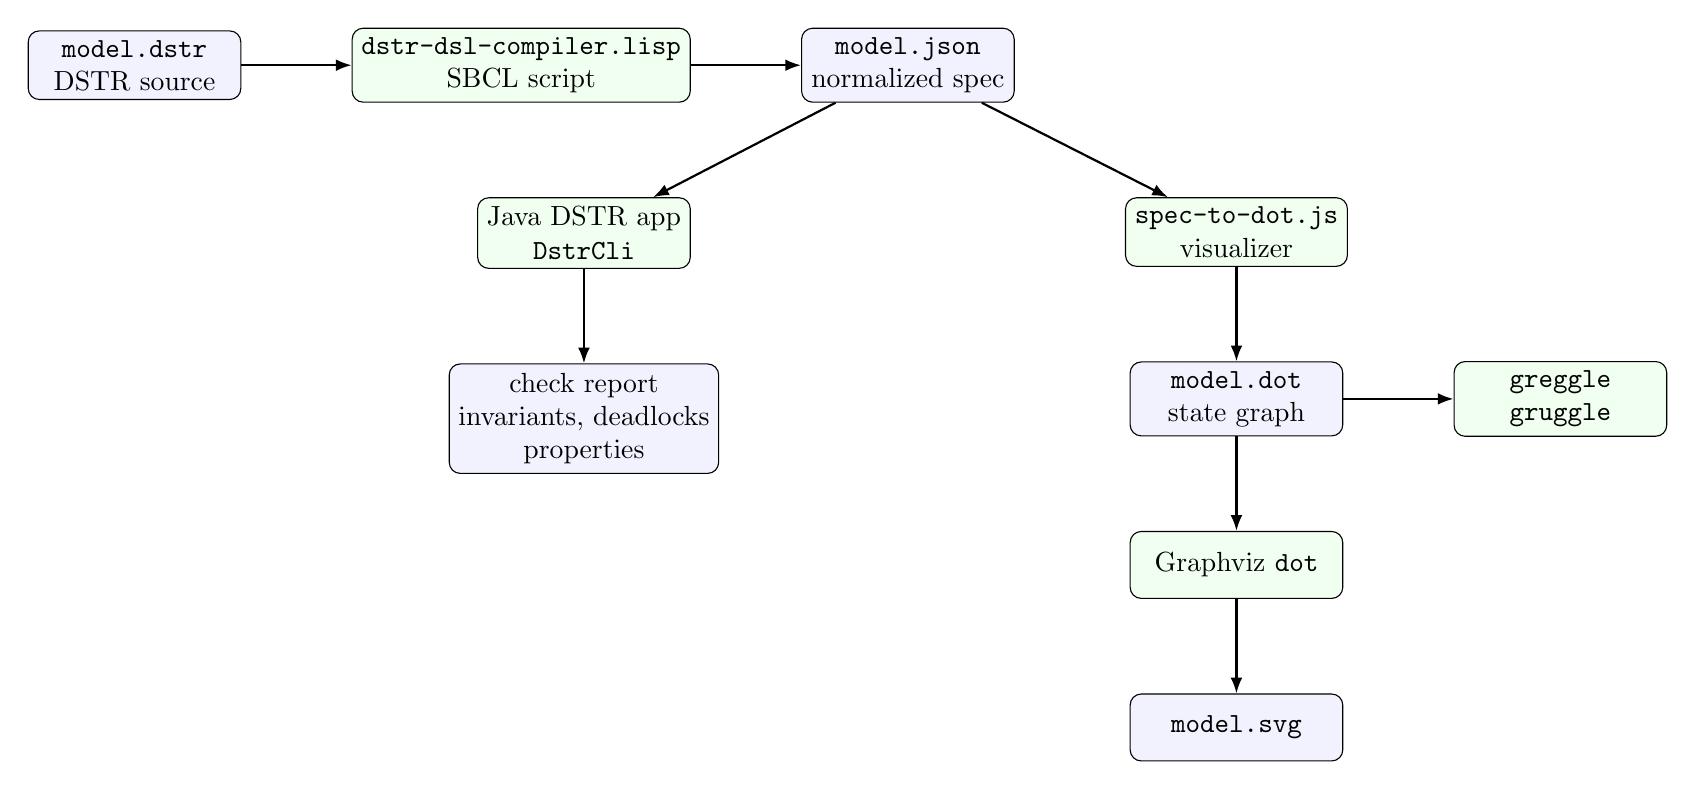
\begin{tikzpicture}[
  node distance=1.2cm and 1.4cm,
  box/.style={draw, rounded corners, align=center, minimum width=2.7cm,
    minimum height=0.85cm, fill=blue!5},
  tool/.style={draw, rounded corners, align=center, minimum width=2.7cm,
    minimum height=0.85cm, fill=green!6},
  arr/.style={-{Latex[length=2mm]}, thick}
]
\node[box] (src) {\texttt{model.dstr}\\DSTR source};
\node[tool, right=of src] (compiler) {\texttt{dstr-dsl-compiler.lisp}\\SBCL script};
\node[box, right=of compiler] (json) {\texttt{model.json}\\normalized spec};
\node[tool, below left=of json] (checker) {Java DSTR app\\\texttt{DstrCli}};
\node[box, below=of checker] (report) {check report\\invariants, deadlocks\\properties};
\node[tool, below right=of json] (dot) {\texttt{spec-to-dot.js}\\visualizer};
\node[box, below=of dot] (dotfile) {\texttt{model.dot}\\state graph};
\node[tool, below=of dotfile] (graphviz) {Graphviz \texttt{dot}};
\node[box, below=of graphviz] (svg) {\texttt{model.svg}};
\node[tool, right=of dotfile] (gg) {\texttt{greggle}\\\texttt{gruggle}};
\draw[arr] (src) -- (compiler);
\draw[arr] (compiler) -- (json);
\draw[arr] (json) -- (checker);
\draw[arr] (checker) -- (report);
\draw[arr] (json) -- (dot);
\draw[arr] (dot) -- (dotfile);
\draw[arr] (dotfile) -- (graphviz);
\draw[arr] (dotfile) -- (gg);
\draw[arr] (graphviz) -- (svg);
\end{tikzpicture}
}
\end{center}

The Java DSTR application is the main model checker.  Use it when the question
is whether invariants hold, whether reachable deadlocks exist, how many
transitions were explored, and whether the recorded existential properties are
true.  The DOT/SVG path is complementary: it gives a visual state graph for
debugging, presentations, and small or bounded state spaces.  The generated
\texttt{.dot} file is also a machine-readable graph artifact that can be fed to
the \texttt{greggle} and \texttt{gruggle} graph interrogation and manipulation
tools.

\section{Command Reference}

\subsection{Compile a Single DSTR File}

The direct compiler script is \texttt{scripts/dstr-dsl-compiler.lisp}.  It
requires SBCL.

\begin{lstlisting}[language=bash]
sbcl --script scripts/dstr-dsl-compiler.lisp \
  dsl-testsuite/light-switch.dstr \
  target/light-switch.json
\end{lstlisting}

On Windows PowerShell:

\begin{lstlisting}[language=bash]
sbcl --script scripts\dstr-dsl-compiler.lisp `
  dsl-testsuite\light-switch.dstr `
  target\light-switch.json
\end{lstlisting}

\subsection{Compile a Directory}

If the input path is a directory, every \texttt{.dstr} file in that directory is
compiled to a corresponding \texttt{.json} file in the output directory.

\begin{lstlisting}[language=bash]
sbcl --script scripts/dstr-dsl-compiler.lisp dsl-testsuite target/dstr-json
\end{lstlisting}

\subsection{Run the Java Model Checker}

After compiling to JSON, run the main Java application from the repository
root.  The Maven and Gradle application entry point is
\texttt{org.dstr.cli.DstrCli}.

\begin{lstlisting}[language=bash]
mvn exec:java -Dexec.args="target/light-switch.json"
gradle run --args="target/light-switch.json"
\end{lstlisting}

The checker parses the normalized JSON, enumerates the finite state universe,
performs reachability from \texttt{init} through \texttt{next}, checks every
invariant on every reachable state, records deadlock paths, and evaluates
\texttt{eventually} properties as reachability summaries.  Its output includes
the spec name, reachable-state count, explored-transition count, property
truth values, invariant counterexample paths, and deadlock paths.

\subsection{Generate DOT and SVG}

The wrapper scripts compile DSTR when needed, run the Node.js graph generator,
and invoke Graphviz.  This is the visualization path, not a replacement for
the Java model-checking CLI.

\begin{lstlisting}[language=bash]
./dstr-to-svg.sh dsl-testsuite/light-switch.dstr
./dstr-to-svg.sh dsl-testsuite/bakery-3proc.dstr --max-states 500
\end{lstlisting}

PowerShell:

\begin{lstlisting}[language=bash]
.\dstr-to-svg.bat dsl-testsuite\light-switch.dstr
.\dstr-to-svg.bat dsl-testsuite\bakery-3proc.dstr --max-states 500
\end{lstlisting}

The wrapper accepts either \texttt{input.dstr} or an already-normalized
\texttt{input.json}.  It writes adjacent \texttt{.json}, \texttt{.dot}, and
\texttt{.svg} files.  The \texttt{.svg} file is for visual inspection; the
\texttt{.dot} file can also be passed to \texttt{greggle} or \texttt{gruggle}
for graph interrogation and manipulation.

\subsection{Graph Options}

Options after the input file are passed to \texttt{scripts/spec-to-dot.js}.

\begin{description}
\item[\texttt{--all-states}] Include unreachable states as dashed gray nodes.
\item[\texttt{--rankdir TB}] Draw top-to-bottom.  Use \texttt{LR} for
  left-to-right.
\item[\texttt{--max-states N}] Truncate a large explicit universe after
  enumerating \texttt{N} states.
\item[\texttt{--compact}] Force compact node labels.
\item[\texttt{--no-legend}] Omit the legend node in compact graphs.
\end{description}

\section{System Form}

Every source file must contain exactly one \texttt{system} form after optional
top-level helper forms.

\begin{lstlisting}[language=DSTR]
(system light-switch
  (vars light)
  (domain light off on)
  (init (= light off))
  (action turn-on
    (= light off)
    (= light+ on))
  (action turn-off
    (= light on)
    (= light+ off))
  (next (or $turn-on $turn-off))
  (invariant type-ok
    (in light (set off on)))
  (property eventually-on
    (eventually (= light on))))
\end{lstlisting}

\subsection{Clauses}

\begin{description}
\item[\texttt{(vars v...)}] Declares state variables in output order.
\item[\texttt{(vars* sep (a...) * (b...))}] Declares the Cartesian product of
  two name groups, joining each pair with \texttt{sep}.
\item[\texttt{(domain v value...)}] Gives \texttt{v} a finite domain.  Multiple
  values are emitted as a set.  A single \texttt{\$EnumName} value expands to
  the symbols loaded from a Java enum type.
\item[\texttt{(domain* glob value...)}] Applies the domain to every declared
  variable whose name matches the glob pattern.
\item[\texttt{(init expr...)}] Defines the initial-state predicate.
\item[\texttt{(action name expr...)}] Defines a named transition predicate.
\item[\texttt{(next expr...)}] Defines the next-state relation, usually as a
  disjunction of action references.
\item[\texttt{(invariant name expr...)}] Defines a predicate checked over every
  reachable state.
\item[\texttt{(property name expr...)}] Defines a property summary.  Currently
  \texttt{eventually} is reachability-style: it is true if some reachable state
  satisfies the body.
\end{description}

When any clause body contains more than one expression, the compiler combines
the body as an implicit \texttt{and}.

\section{Names, Literals, and State Variables}

\begin{description}
\item[Current variable] A declared variable name such as \texttt{pc} compiles to
  \texttt{\{"var": "pc"\}}.
\item[Next variable] A declared variable with a trailing \texttt{+}, such as
  \texttt{pc+}, compiles to \texttt{\{"next": "pc"\}}.  Next variables are
  valid in actions and in \texttt{next}.
\item[Action reference] \texttt{\$turn-on} and the older \texttt{@turn-on}
  compile to \texttt{\{"actionRef": "turn-on"\}} inside \texttt{next}.
\item[Symbol literal] A bare undeclared symbol such as \texttt{off} compiles as
  the string literal \texttt{"off"}.
\item[Number literal] Numbers remain numeric.
\item[Boolean literal] \texttt{t} and \texttt{nil} compile as true and false.
\item[Quoted literal] \texttt{'foo} or \texttt{(quote foo)} forces a literal
  value.
\end{description}

\section{Expression Reference}

\subsection{Logical Operators}

\begin{lstlisting}[language=DSTR]
(and (= pc idle) (= flag false))
(or $enter $exit)
(not (= pc cs))
(implies (= pc cs) (= lock held))
\end{lstlisting}

\subsection{Equality, Comparison, and Arithmetic}

\begin{lstlisting}[language=DSTR]
(= count 0)
(!= mem 0)
(< ticket other-ticket)
(<= hr 12)
(= count+ (+ count 1))
(= remaining+ (- remaining 1))
\end{lstlisting}

The arithmetic operators \texttt{+}, \texttt{-}, \texttt{*}, and \texttt{/}
compile to JSON arithmetic nodes.  Division is integer division in the
JavaScript graph evaluator.

\subsection{Sets and Membership}

\begin{lstlisting}[language=DSTR]
(domain pc idle trying cs)
(in pc (set idle trying cs))
(= allowed (set a b c))
\end{lstlisting}

In a \texttt{domain} clause, a sequence of values is automatically treated as a
set.  Use \texttt{(set ...)} when a set is needed inside an expression.

\subsection{Domains from Java Enums}

Java enum declarations can be loaded before the \texttt{system} form.  Each
argument to \texttt{load-java-enums} may be a \texttt{.java} file or a directory;
directories are searched recursively for Java source files.  The enum scanner is
intentionally lightweight and is aimed at ordinary declarations such as
\texttt{public enum Lifecycle \{ NEW, READY, DISABLED \}}.

\begin{lstlisting}[language=DSTR]
(load-java-enums "src/main/java")

(system lifecycle-model
  (vars state)
  (domain state $Lifecycle)
  (init (= state new))
  (action activate
    (= state new)
    (set state as ready))
  (next $activate))
\end{lstlisting}

DSTR normalizes symbols to lower-case strings, so Java constants such as
\texttt{NEW} and \texttt{READY} are used as \texttt{new} and \texttt{ready} in
the model.

\subsection{Domains from Protocol Buffer Enums}

Protocol buffer enum declarations can be loaded before the \texttt{system} form
with \texttt{load-proto-enums}.  Arguments may be \texttt{.proto} files or
directories, and directories are searched recursively.  The loader recognizes
ordinary protobuf enum entries of the form \texttt{NAME = number;} and ignores
enum options, reserved declarations, comments, and option values.

\begin{lstlisting}[language=DSTR]
(load-proto-enums "src/main/proto")

(system order-model
  (vars status)
  (domain status $OrderStatus)
  (init (= status order_status_new))
  (action ready
    (= status order_status_new)
    (set status as order_status_ready))
  (next $ready))
\end{lstlisting}

As with Java enums, DSTR normalizes protobuf enum symbols to lower-case strings.

\subsection{Quantifiers}

\begin{lstlisting}[language=DSTR]
(forall (p in (set p1 p2 p3))
  (in p (set p1 p2 p3)))

(exists (owner in (set p1 p2))
  (= owner lock-owner))
\end{lstlisting}

The quantified variable is local to the body.

\subsection{Temporal Property Form}

\begin{lstlisting}[language=DSTR]
(property p1-can-reach-cs
  (eventually (= p1pc cs)))
\end{lstlisting}

The prototype treats this as an existential reachability question over the
reachable state graph, not as a full temporal-logic liveness proof.

\section{Transition Shorthands}

\subsection{Assignment}

These three forms are equivalent in an action body:

\begin{lstlisting}[language=DSTR]
(= light+ on)
(assign on to light)
(set light as on)
\end{lstlisting}

They all assert equality between the next state of \texttt{light} and the value
\texttt{on}.

\subsection{Unconditional Transitions}

An action does not need an \texttt{if ... then ...} guard.  If a transition is
unconditional, write the next-state assignments directly in the action body:

\begin{lstlisting}[language=DSTR]
(action reset
  (assign IDLE to pc)
  (set count as 0)
  (assign nil to busy))
\end{lstlisting}

This is equivalent to writing the next-state equalities explicitly:

\begin{lstlisting}[language=DSTR]
(action reset
  (= pc+ IDLE)
  (= count+ 0)
  (= busy+ nil))
\end{lstlisting}

If some variables should stay unchanged, include frame conditions in the same
action body:

\begin{lstlisting}[language=DSTR]
(action reset
  (assign IDLE to pc)
  (set count as 0)
  (!unchanged owner mode))
\end{lstlisting}

or with glob-based sugar:

\begin{lstlisting}[language=DSTR]
(action reset
  (assign IDLE to pc)
  (set count as 0)
  (unchanged* *_status *_version))
\end{lstlisting}

Any next-state variable left unconstrained by an action may take any value in
its domain in the candidate successor state, so deterministic-looking actions
should assign or frame every relevant variable.

\subsection{Equality Alias}

\begin{lstlisting}[language=DSTR]
(equals p_settlement_state OPEN)
\end{lstlisting}

is equivalent to:

\begin{lstlisting}[language=DSTR]
(= p_settlement_state OPEN)
\end{lstlisting}

\subsection{Conditional Form}

\begin{lstlisting}[language=DSTR]
(if
  ((equals p_settlement_state OPEN)
   (equals c1_settlement_state OPEN))
  then
  ((assign CANCELLED to p_settlement_state)
   (assign CANCELLED to c1_settlement_state)))
\end{lstlisting}

The conditional shorthand means conjunction of the condition and consequence.
It is not a branching expression with an \texttt{else}; it is useful for
writing guarded transition cases.  A branch written as a list of sibling
expressions is treated as an implicit \texttt{and}.

\subsection{Frame Conditions by Glob}

\begin{lstlisting}[language=DSTR]
(unchanged* *_market_status *_event_type *_mission_version)
\end{lstlisting}

This expands to a conjunction of frame equalities for every declared variable
matched by the glob patterns:

\begin{lstlisting}[language=DSTR]
(and (= p_market_status+ p_market_status)
     (= c1_market_status+ c1_market_status)
     ...)
\end{lstlisting}

\subsection{Alternate Scenarios}

\begin{lstlisting}[language=DSTR]
(alternate-scenarios
  (if (= state OPEN) then (assign CANCELLED to state))
  (if (= state BOOKED) then (assign state to state)))
\end{lstlisting}

\texttt{alternate-scenarios} is a readability alias for \texttt{or}.

\section{Macros and Helper Functions}

DSTR permits top-level \texttt{defmacro}, \texttt{defun}, \texttt{load},
\texttt{load-java-enums}, and \texttt{load-proto-enums} forms before the
\texttt{system}.  Relative paths are resolved against the current
\texttt{.dstr} file's directory.

\subsection{Expansion Forms}

\begin{description}
\item[\texttt{(expand name arg...)}] Macroexpand a named macro.
\item[\texttt{(\%name arg...)}] Shorthand for \texttt{(expand name arg...)}.
\item[\texttt{(!name arg...)}] Expand a macro whose result is a list of sibling
  forms and splice those forms into the surrounding body.
\end{description}

\subsection{Built-in Macro Helpers}

\begin{lstlisting}[language=DSTR]
(%same pc)              ; expands to (= pc+ pc)
(!unchanged p2pc mem)   ; splices (= p2pc+ p2pc), (= mem+ mem)
\end{lstlisting}

\subsection{Example Macro Library}

\begin{lstlisting}[language=DSTR]
(defun preserve-clauses (&rest vars)
  (mapcar (lambda (var)
            `(= ,(next-var-symbol var) ,var))
          vars))

(defmacro preserve (&rest vars)
  (preserve-clauses vars))
\end{lstlisting}

\subsection{CAS Race With Spliced Actions}

\begin{lstlisting}[language=DSTR]
(defmacro p1-actions ()
  '((action p1-start
      (= p1pc a0)
      (= p1pc+ try)
      (!preserve p2pc mem))
    (action p1-cas-success
      (= p1pc try)
      (= mem 0)
      (= p1pc+ won)
      (!preserve p2pc)
      (= mem+ 1))))

(system cas-2proc-race
  (vars p1pc p2pc mem)
  (domain p1pc a0 try won lost)
  (domain p2pc a0 try won lost)
  (domain mem 0 1 2)
  (init (= p1pc a0) (= p2pc a0) (= mem 0))
  (!p1-actions)
  (next (or $p1-start $p1-cas-success)))
\end{lstlisting}

\section{Product Variables and Glob Domains}

\begin{lstlisting}[language=DSTR]
(system trade-cancellation
  (vars* _ (p c1 c2) * (market_status settlement_state settlement_version))
  (domain* *_market_status MATCHED)
  (domain* *_settlement_state OPEN RELEASED BOOKED CANCELLED)
  (domain* *_mission_version 1 2 3)
  (init
    (equals p_settlement_state OPEN)
    (equals c1_settlement_state OPEN)
    (equals c2_settlement_state OPEN))
  ...)
\end{lstlisting}

The \texttt{vars*} clause above declares:
\[
\texttt{p\_market\_status},\ \texttt{p\_mission\_state},\ldots,
\texttt{c2\_mission\_version}.
\]

\section{Visualization Semantics}

The graph tool enumerates the finite state universe, finds states satisfying
\texttt{init}, applies \texttt{next}, and annotates the reachable graph.

\begin{center}
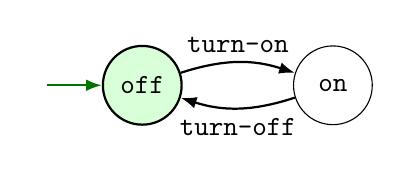
\begin{tikzpicture}[
  node distance=1.4cm,
  state/.style={circle, draw, minimum size=1cm, align=center},
  init/.style={state, fill=green!15, thick},
  dead/.style={state, fill=yellow!20, thick},
  bad/.style={state, fill=red!15, thick},
  arr/.style={-{Latex[length=2mm]}, thick}
]
\node[init] (off) {\texttt{off}};
\node[state, right=of off] (on) {\texttt{on}};
\node[left=0.7cm of off] (start) {};
\draw[arr, green!45!black] (start) -- (off);
\draw[arr] (off) to[bend left=18] node[above] {\texttt{turn-on}} (on);
\draw[arr] (on) to[bend left=18] node[below] {\texttt{turn-off}} (off);
\end{tikzpicture}
\end{center}

Green nodes are initial states, amber nodes are deadlocks, and red nodes are
states where at least one invariant fails.  Edge labels name the actions that
were enabled for that transition.

\section{Normalized JSON Shape}

The compiler emits JSON in the same shape as the core checker expects:

\begin{lstlisting}[language=JSON]
{
  "name": "light-switch",
  "variables": ["light"],
  "domains": {
    "light": {
      "set": [{"lit": "off"}, {"lit": "on"}]
    }
  },
  "init": {
    "=": [{"var": "light"}, {"lit": "off"}]
  },
  "actions": [
    {
      "name": "turn-on",
      "body": {
        "and": [
          {"=": [{"var": "light"}, {"lit": "off"}]},
          {"=": [{"next": "light"}, {"lit": "on"}]}
        ]
      }
    }
  ],
  "next": {"or": [{"actionRef": "turn-on"}, {"actionRef": "turn-off"}]},
  "invariants": [],
  "properties": []
}
\end{lstlisting}

\section{Practical Modelling Notes}

\begin{itemize}
\item Every variable must have exactly one domain, either through
  \texttt{domain} or \texttt{domain*}.
\item Actions should usually define every next-state variable, directly or via
  a frame condition.  If a variable is not constrained, the explicit-state
  checker may allow many successor values.
\item Use \texttt{unchanged}, \texttt{unchanged*}, or \texttt{same} to make
  frame conditions visible and auditable.
\item Keep large product domains small while exploring a model.  Use
  \texttt{--max-states} for graphing large universes.
\item Prefer \texttt{\$action} for new Lisp-style models.  The older
  \texttt{@action} form remains accepted for compatibility.
\end{itemize}

\section{Minimal Checklist}

\begin{enumerate}
\item Declare variables with \texttt{vars} or \texttt{vars*}.
\item Provide finite domains for all variables.
\item Define an \texttt{init} predicate.
\item Define one or more \texttt{action} clauses.
\item Define \texttt{next}, normally as an \texttt{or} of action references.
\item Add invariants and reachability properties.
\item Compile to JSON, run the Java DSTR checker for the authoritative checking
  report, then use \texttt{spec-to-dot.js} or the SVG wrapper for graph
  inspection.
\end{enumerate}

\end{document}
